\chapter{第五關:迴圈}

%1
\section{A007\&A022 - 最大公因數}
輸入兩個正整數x, y,輸出x, y的最大公因數。

\subsection{解題思惟}
求最大公因數有很多方法,這裡先講解一個簡單的暴力法,主要的概念是從最大的可能值往下找,找到的第一個共同的因數就是最大公因數。
\begin{enumerate}
\item 假設x<y,如果不是的話,將兩個數交換。最大公因數不會大於x。
\item 跑一迴圈變數i從x到1,第一個發現是x和y的公因數的i就是最大公因數。
\item 其實第一點可以省略,只是當x很大而y很小的時候,會多跑很多次迴圈而已。
\end{enumerate}

\subsection{程式碼}
\begin{cppcode}
#include <iostream>

using namespace std;

int main()
{
	int x, y, i;
	cin >> x >> y;
	for (i=x; i>=1; i--) {
		if (x%i==0 && y%i==0) break;
	}
	cout << i;
	return 0;
}
\end{cppcode}

\subsection{解題思惟}
接著要講述的方法是輾轉相除法。
\begin{enumerate}
\item 如果x除以y整除的話,那麼y就是最大公因數。
\item 如果不能整除的話,可以先算出x除以y的餘數,這個數肯定比y還小,接著把y變成新的x,把剛才的餘數變成新的y,再回到上一個步驟。
\end{enumerate}
\subsection{程式碼}
\begin{cppcode}
#include <iostream>

using namespace std;

int main()
{
	int x, y, t;
	cin >> x >> y;
	while (x%y) { // x % y != 0
		x = x%y;
		t=x; x=y; y=t; // swap(x, y);
	}
	cout << y;
	return 0;
}
\end{cppcode}
註:本題在瘋狂程設測試時,沒有辦法通過。仔細檢查,發現輸入的數有的是負數,不像題目所說的都是正整數,因此會產生錯誤。修正的辦法,是在輸入x, y整數之後,加上負數的判斷並改成正數,也就是下面兩行:
\begin{inside}
if (x<0) x = -x;
if (y<0) y = -y;
\end{inside}
這樣的話,就沒有問題了。

%2
\section{A008 - 九九乘法表}
請如同範例程式印出九九乘法表。
\begin{figure}[H]
	\centering
	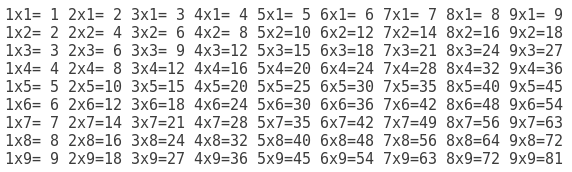
\includegraphics[width=0.9\textwidth]{fig/L5_example_001}
	\label{L5_example_001}
\end{figure}

\subsection{解題思惟}
\begin{enumerate}
	\item 使用兩個for迴圈,第一個用來印出乘號後面的數字,第二個用來印出乘號前面的數字。
	\item 此題需要注意的是,為了使九九乘法表對齊,乘出來的數字要佔兩個位置,因此小於十的乘積需在十位數的地方補一個空格。這個部份使用printf較為簡單,直接使用\%2d的指定格式即可。
\end{enumerate}

\subsection{程式碼}
\begin{cppcode}
	#include <cstdio>
	
	int main()
	{
		for(int i=1; i<10; i++) {
			for(int j=1; j<10; j++) {
				printf("%dx%d=%2d ", j, i, i*j);
			}
			printf("\n");
		}
		return 0;
	}
\end{cppcode}
註:本題在瘋狂程設測試時,限制不能出現\",因此上述程式沒有辦法通過。因為printf第一個參數是字串,會用到\",那我們可以改用cout,然後其他文字都改用字元(字元使用\'而不是\"),這樣的話,程式碼可以改寫如下:
\begin{inside}
	#include <iostream>
	#include <iomanip>
	
	using namespace std;
	
	int main()
	{
		for(int i=1; i<10; i++) {
			for(int j=1; j<10; j++) {
				cout<<j<<'x'<<i<<'='<<setw(2)<<i*j<<' ';
			}
			cout<<endl;
		}
		return 0;
	}
\end{inside}
注意此處輸出乘積的時候,限制輸出寬度為2格,可以引入<iomanip>檔頭,並在cout中使用setw(2)的敘述達成。或者也可以自行判斷,當乘積小於10的時候,先多印一個空白,再輸出乘積。

%3
\section{A009 - 質數判別}
輸入一個正整數,如果是質數,則輸出 Yes,如果不是,則輸出 No。

\subsection{解題思惟}
\begin{enumerate}
\item 質數的特色是除了1之外,另外一個唯一的因數就是n本身。所以從1檢查到n,應該有2個因數。以下的程式應該就可以判斷了。
	\begin{inside}
	int cnt=0;
	for (i=1; i<=n; i++) if (n%i==0) cnt++; // 檢查到因數,把個數加1。
	if (cnt==2) cout<<"Yes"; else cout<<"No";
	\end{inside}
\item 也可以只檢查2, …, n-1是否為n的因數,如果其中有一個因數,那n就不是質數了,否則n就是質數。在這種情況下,1和2應該要另外處理,1不是質數,但2是質數。
\item 可以設定一個旗標變數,如果沒有因數存在,把值設為1 (表示n為質數),當有任一個因數存在時,把它設為0 (表示n非質數)。預設值可以為1,檢查到因數時設為0。像以下這樣:
	\begin{inside}
	int flag=1;
	for (i=2; i<n; i++) if (n%i==0) { flag=0; break; }
	\end{inside}
\item 綜合2-3兩點,也可以用以下方式解此問題。
	\begin{inside}
	int flag=1; // 預設flag為1
	if (n==1) flag=0; // 1不是質數
	else if (n>3) { // 2和3是質數,flag不用變動,處理n>3情況即可
		for (i=2; i<n; i++) if (n%i==0) { flag=0; break; }
	}
	\end{inside}
\item  進階思考:實際上檢查$n$的因數只要檢查到$\sqrt{n}$即可,因為如果有個因數$x$超過$\sqrt{n}$,那麼$n/x$就小於$\sqrt{n}$,會先被檢查到。另外$i\le\sqrt{n}$可以改成$i*i\le n$。
\item 偶數不是質數,也可以先過濾掉,奇數的部份,只要檢查有沒有奇數的因數就可以了。
\end{enumerate}

\subsection{程式碼}
\begin{cppcode}
	#include <iostream>
	
	using namespace std;
	
	int main()
	{
		int i, n, flag=1;
		cin >> n;
		if (n==1) flag=0; // 1 非質數
		else if (n>3) { // 2和3是質數,flag不用變動,處理n>3情況即可
			if (n%2==0) flag=0; // 偶數非質數
			else for (i=3; i*i<=n; i+=2) { // 只檢查奇數i,範圍i*i<=n
				if (n%i==0) { flag=0; break; } // 發現因數,設定旗標跳出
			}
		}
		if (flag) cout << "Yes";
		else cout << "No";
		return 0;
	}
\end{cppcode}

%4
\section{A012 - 標準分解式}
輸入一正整數$N$, $N\ge 2$,輸出$N$的標準分解式。例如輸入12,則輸出2*2*3。

\subsection{解題思惟}
\begin{enumerate}
	\item 考慮因數的時候,設$p$從2開始一直到$N$,可以一一嘗試,看$p$是否為$N$的因數。
	\item 如果找到一個因數$p$,有可能$N$的這個因數有很多個,例如12有2個2的因數,所以當找到因數$p$的時候,把$N$變成$N/p$,再繼續嘗試看看除以$p$之後的$N$值是否還有$p$的因數,要一直試到沒有$p$的因數為止,然後再繼續檢查下一個數$p+1$。這可以寫一個while迴圈來處理,只要$p$還是$N$的因數,就一直除下去,把所有$p$的因數找出來,像下面這樣:
	\begin{inside}
	for (int p=2; p<=n; p++) {
		while (N%p == 0) {
			cout << "*" << p; 
			N /= p; 
		}
	}
	\end{inside}
	\item 或者另一個方法,就是當找到$p$是$N$的因數的時候,除了輸出$p$並且把$N$變成$N/p$之外,在主迴圈裡面不要把$p$加1,這樣重覆下一次迴圈的時候,$p$就會再被測試一次,這樣就可以把所有的因數$p$找出來。但是當$p$不是$N$的因數的時候,要記得把$p$加1,這樣才能繼續測試下一個數,像下面這樣:
	\begin{inside}
	for (int p=2; p<=n; ) { // 注意沒有更新式 p++
		if(n%p == 0) { // p是n的因數
			cout << "*" << p;
			n /= p; // 把因數p除掉,p仍維持原來的值
		} else p++; // p不是因數,把p加1
	}
	\end{inside}
	\item 如果$p<N$且$p$是$N$的因數,那麼$p$的因數也會是$N$的因數,所以在嘗試到$p$之前,$p$的因數應該都已經被找過了,而且更新過的$N$也已經除掉了所有$p$的因數。換句話說,當找到$p$是$N$的因數的時候,$p$應該沒有1和$p$以外的因數了,也就是$p$應該是質數,這樣一來,透過上面的程序,只要找到的$p$是$N$的因數,那一定也是質因數了。
	\item 第一個質因數不需要列印*號,其他的因數在列印之前要加上一個*號。這可以宣告一個first變數,一開始設為1,當列印過因數後,就把它設成0,然後在列印的時候,如果first為1,就不用列印*號,否則都要先列印*號。
\end{enumerate}
\subsection{程式碼}
\begin{cppcode}
#include <iostream>

using namespace std;

int main()
{
	int n, first=1;
	cin >> n;
	for (int p=2; p<=n; ) {
		if(n%p == 0) { // p是n的因數
			if(first) { cout<<p; first=0; }
			else cout << "*" << p;
			n /= p; // 把因數p除掉,p仍維持原來的值
		} else p++; // p不是因數,把p加1
	}
	return 0;
}
\end{cppcode}

%5
\section{A013 - 年月日算第幾天}
輸入西元年月日,算該日是該年的第幾天。

\subsection{解題思惟}
\begin{enumerate}
	\item 將每月的天數存在陣列中。陣列可宣告13個,第0個元素不用,第1到12個元素分別表示1月到12月的天數,這樣使用起來會比較便利。
	\item 先計算該年為平年或閏年。基本上每4年閏一次,但每100年少一次,每400年又要加回一次。可用以下方式檢查:
	\begin{inside}
	if (y%4==0) leap = true;
	if (y%100==0) leap = false;
	if (y%400==0) leap = true;
	\end{inside}
	或者也可以使用以下方式:
	\begin{inside}
	leap = false;
	if (y%400==0) leap = true;
	else if (y%100!=0 && y%4==0) leap = true;
	\end{inside}
	\item 2月的天數先以28天計算,如果是閏年的話,把它加1。
	\item 假設輸入的月和日分別為m和d,將1至m-1月的天數加起來,再加上d就是答案了。
	\item 本題如果不用陣列的話,也可以使用switch來解題,第m月的天數可用以下程式碼決定:
	\begin{inside}
	switch (m) {
	case 1:case 3:case 5:case 7:case 8:case 10:case 12: days=31; break;
	case 4:case 6:case 9:case 11: days=30; break;
	case 2: if(leap) days=29; else days=28;
	}
	\end{inside}
\end{enumerate}

\subsection{程式碼}
\begin{cppcode}
#include <iostream>

using namespace std;

int main()
{
	int month[13]={0,31,28,31,30,31,30,31,31,30,31,30,31};
	int yy, mm, dd, i, day=0;
	cin >> yy >> mm >> dd;
	
	if (yy%400==0) month[2]++;
	else if (yy%100!=0 && yy%4==0) month[2]++;
	for (i=1; i<mm; i++) day += month[i];
	day += dd;
	cout << day;
	return 0;
}
\end{cppcode}

%6
\section{A015 - 破解乘法}
輸出所有五位數abcde,該數滿足以下十進位乘法: (abcde)*(a)=(bbbbbe),
其中a不為0且(abcde)=$a*10^4+b*10^3+c*10^2+d*10+e*1$ ,
而 (bbbbbe)=$b*111110+e$。

\subsection{解題思惟}
\begin{enumerate}
	\item 使用for迴圈把abcde的所有可能都試過一次:
\begin{inside}
	for (int a=1; a<10; a++)
		for(int b=0; b<10; b++)
			for(int c=0; c<10; c++)
				for(int d=0; d<10; d++)
					for(int e=0; e<10; e++) { 
						...
\end{inside}
	\item 上面的5個for也可以改成1個for,但是數字要從10000到99999,且需要在迴圈內把a, b, c, d, e分別先算出來,如下:
	\begin{inside}
		for (int abcde=10000; abcde<=99999; abcde++) {
			a = abcde/10000;       // a是萬位,等於除以10000的商
			b = (abcde/1000) % 10; // b是千位,等於除以1000的商的個位
			c = (abcde/100) % 10;  // c是百位,等於除以100的商的個位
			d = (abcde/10) % 10;   // d是十位,等於除以10的商的個位
			e = abcde % 10;        // e是個位,等於除以10的餘數
			...
		}
	\end{inside}
	\item 在每一次迴圈中,檢查該數是否滿足條件?滿足的話就印出來。
\begin{inside}
	int n = a*10000 + b*1000 + c*100 + d*10 + e;
	int m = 111110*b + e;
	if (n*a == m) cout << a << b << c << d << e << endl;
\end{inside}
\end{enumerate}

\subsection{程式碼}
本題因為對於0和1有限制出現次數,並且其餘數字都不能出現,所以使用第一種方式作答。
\begin{cppcode}
#include <cstdio>

int main()
{
	for (int a=1; a<10; a++)
		for(int b=0; b<10; b++)
			for(int c=0; c<10; c++)
				for(int d=0; d<10; d++)
					for(int e=0; e<10; e++) { 
						int abcde = a*10000+b*1000+c*100+d*10+e;
						int bbbbbe = 111110*b+e;
						if(abcde*a == bbbbbe) printf("%d %d %d %d %d",a,b,c,d,e);
					}
	return 0;
}
\end{cppcode}

%7
\section{A020 - 韓信點兵}
韓信點兵, 7個一數剩3個, 9個一數剩4個, 10個一數剩2個, 11個一數剩1個, 請問韓信兵團至少有多少人?

\subsection{解題思惟}
\begin{enumerate}
	\item 因為要求最少可能的人數,所以可從1開始往上嘗試,當條件滿足時即可印出並離開迴圈。
	\item 在判斷條件時,可以使用 \&\& 把幾個條件串起來,全部符合時印出並跳出;或者個別測試,不符合時跳過。前者的用法如下:
	\begin{inside}
		if (i%7==3 && i%9==4 && i%10==2 && i%11==1) { ... }
	\end{inside}
	後者的用法如下:
	\begin{inside}
		if (i%7!=3) continue;
		if (i%9!=4) continue;
		if (i%10!=2) continue;
		if (i%11!=1) continue;
		...
	\end{inside}
\end{enumerate}


\subsection{程式碼}
\begin{cppcode}
	#include <iostream>
	
	using namespace std;
	
	int main() 
	{
		for (int i=1; ; i++) {
			if (i%7==3 && i%9==4 && i%10==2 && i%11==1) {
				cout << i;
				break;
			}
		}
		return 0;
	}
\end{cppcode}


%8
\section{A021 - N階乘}
輸入一個正整數n,輸出n!。

\subsection{解題思惟}
n!等於從1乘到n,可使用一個變數m,將初始值設為1,並累乘至輸入的正整數n即可。

\subsection{程式碼}
\begin{cppcode}
	#include <iostream>
	
	using namespace std;
	
	int main()
	{
		int n, m=1;
		cin >> n;
		for (int i=1; i<=n; i++) m *= i;
		cout << m;
		return 0;
	}
\end{cppcode}

%\section{最大公因數} 前面已做過
%10梁
\section{A023 - 比N小的質數}
輸入一正整數N,輸出比N小的所有質數。

\subsection{解題思惟}
\begin{enumerate}
	\item 前面已處理過判別質數的問題,可以把它寫成一個函式,輸入n,輸出為1或0,1表示質數,0表示非質數。
	\item 把小於N的所有數字跑一遍,用上面的函式檢查是否為質數即可。
\end{enumerate}

\subsection{程式碼}
\begin{cppcode}
#include <iostream>

using namespace std;

int isprime(int n);

int main()
{
	int n;
	cin >> n;
	for (int i=2; i<n; i++) {
		if (isprime(i)) cout << i << " ";
	}
	return 0;
}

int isprime(int n)
{
	if (n<=1) return 0;
	if (n<4) return 1; // 2 and 3 are primes
	if (n%2==0) return 0; // 偶數非質數
	for (int i=3; i*i<=n; i+=2) {
		if (n%i==0) return 0;
	}
	return 1;
}
\end{cppcode}

%11梁
\section{A024 - 級數}
輸入一正整數N。輸出$1*3+3*5+5*7+...+(2N-1)(2N+1)$之值。

\subsection{解題思惟}
\begin{enumerate}
\item 初始化變數ans等於0,用來做為累加之用。
\item 跑迴圈令i從1到2n-1,每次把i*(i+2)加到ans即可。
\end{enumerate}

\subsection{程式碼}
\begin{cppcode}
#include <iostream>

using namespace std;

int main()
{
	int N, ans = 0;
	cin >> N;
	for (int i=1; i<=2*N-1; i+=2) {
		ans += i*(i+2);
	}
	cout << ans;
	return 0;
}
\end{cppcode}

%12梁
\section{A026 - 七進位轉十進位}
輸入5個七進位字母,輸出該數的十進位表達。

\subsection{解題思惟}

\begin{enumerate}
	\item 輸入整數n。因為七進位的字母都是數字,所以可用整數讀取。
	\item 初始化變數ans等於0,準備進行累加。
	\item 初始化變數k等於1 $(=7^0)$,k用來表示$7^i$之值,所以下面跑迴圈時每次都要乘以7。
	\item 用for迴圈進行五次七進位轉十進位的運算,每次都取n的個位數乘上k,將其累加到ans上,然後將n除以10,以便把處理過的個位去掉。
	\begin{inside}
	for (i=0; i<5; i++) {
		ans += (n%10*k);
		n /= 10;
		k *= 7;
	}
	\end{inside}
\end{enumerate}

\subsection{程式碼}
\begin{cppcode}
#include <stdio.h>

int main()
{
	int n, ans = 0;
	scanf("%d", &n);
	int k = 1;
	for(int i=0; i<5; i++) {
		ans += (n%10*k);
		n /= 10;
		k *= 7;
	}
	printf("%d", ans);
	return 0;
}
\end{cppcode}

%13梁
\section{A027 - 十六進位轉十進位}
輸入5個十六進位字母 0...9A...F,輸出輸出該數的十進位。

\subsection{解題思惟}
\begin{enumerate}
	\item 第一次讀一個字元,算出其十進位的值,接著讀第二個字元,算出該兩個字元十進位的值,依此類推,最後可以得到答案。
	\item 單一個字元轉成十進位的話,如果是0-9,值也是0-9,如果是A-F,值是10-15。所以當字元為0-9時,將字元減去`0'字元就可以得到相對的數目,如果是文字的話,減掉`A'字元加上10,就可以得到相對的數目。文字的部份,要注意大小寫。
	\item 將前一次所算出的結果乘以16,加上新進來的個位數,就可以得到下一個更新的值。總共重覆5次,就可以得到答案。
\end{enumerate}

\subsection{程式碼}
\begin{cppcode}
	#include <iostream>
	using namespace std;
	int main()
	{
		int ans=0;
		char c;
		for(int i=0; i<5; i++) {
			cin >> c;
			ans *= 16;
			if (c>='0' && c<='9') ans += c-'0';
			else if (c>='A' && c<='F') ans += c-'A'+10;
			else if (c>='a' && c<='f') ans += c-'a'+10;
		}
		cout<<ans;
		return 0;
	}
\end{cppcode}

%14梁
\section{A028 - 十進位轉七進位}
輸入一個正整數N,輸出該數的七進位表達式。

\subsection{解題思惟}
\begin{enumerate}
	\item 十進位整數可以直接讀取。轉成七進位時,一般作法是把該數除以7,得到的餘數為最末位,商的部份繼續除以7,得到的餘數為次末位,依此類推,至不能再除為止。
	\item 因為得到的位數是從個位開始到最高位,但輸出是要倒過來,所以要先把得到的值存起來,最後倒過來輸出。存起來的方式可以使用陣列。
	\item 本題也可以從最高位算起,但是要先計算最高位的權重(即7的最高次冪)。計算的方式,是從權重1開始,每次把權重乘以7,一直到大於該數大小之前,此即為最高位。
	\item 設最高位權重為d,則該數n除以d即得到最高位數,其次將d除以7,得到次高位權重,將n除以該權重,然後再求7的餘數得次高位數,依此類推。使用本方法計算的話,可以逐位輸出,不需要先儲存每一位的數字。
\end{enumerate}

\subsection{程式碼}
一般解法
\begin{cppcode}
#include <stdio.h>

int main()
{
	int n, a[20], idx=0;
	scanf("%d", &n);
	while (n) { a[idx++]=n%7; n/=7; }
	for (n=idx-1; n>=0; n--) printf("%d", a[n]);
	return 0;
}
\end{cppcode}
	
由高位起首解法
\begin{cppcode}
#include <stdio.h>

int main()
{
	int n, d=1;
	scanf("%d", &n);
	while (d<=n) d*=7;
	for (d/=7; d; d/=7) printf("%d", n/d%7);
	return 0;
}    
\end{cppcode}

%15梁
\section{A029 - 費式數列}
費氏數列定義如下 $f(0)=0, f(1)=1, f(n)=f(n-1)+f(n-2)$;請從螢幕輸入一個正整數n,輸出$f(n)$。

\subsection{解題思惟}

\begin{enumerate}
\item 本題可以使用遞迴或非遞迴方式求解。先討論遞迴寫法。
\item 遞迴函式f(n),如果n<2,回傳n即可,n>=2時,回傳f(n-1)+f(n-2)即可。
\item 如果不使用遞迴的話,可以設fn, fnm1, fnm2三個變數,分別表示f(n), f(n-1)及f(n-2),先設好f(n-1)及f(n-2)的初始值,然後每次計算fn=fnm1+fnm2,算完後令 fnm2=fnm1, fnm1=fn,不斷重覆即可,重覆次數為n-1次。
\end{enumerate}

\subsection{程式碼}
遞迴版本
\begin{cppcode}
#include <cstdio>

int f(int n);

int main()
{
	int n;
	scanf("%d", &n);
	printf("%d", f(n));
	return 0;
}

int f(int n)
{
	if (n<2) return n;
	return f(n-1)+f(n-2);
}
\end{cppcode}
非遞迴版本
\begin{cppcode}
#include <cstdio>

int main()
{
	int n, fn, fnm1=1, fnm2=0;
	scanf("%d", &n);
	if (n<2) fn=n;
	else for (int i=2; i<=n; i++) {
		fn = fnm1 + fnm2;
		fnm2 = fnm1;
		fnm1 = fn;
	}
	printf("%d", fn);
	return 0;
}
\end{cppcode}

%16梁
\section{A045 - 大樂透包牌}
大樂透從1到49號中選6個號碼,開獎時共開出6個號碼及1個特別號,6個號碼全中者得頭獎。
阿平每期計算明牌,挑出8個號碼,想要將所有由這8個號碼所組的6個號碼全部簽。
請你設計程式供阿平輸入此8個號碼,然後印出所有的簽牌可能。

\subsection{解題思惟}

\begin{enumerate}
\item 將八個數讀到陣列裡。
	\begin{inside}
	int n[8];
	for(int i=0; i<8; i++) {
		scanf("%d", &n[i]);
	}
	\end{inside}
\item 每次剔除兩個數,輸出其他六個數。假設a和b是要剔除的數的索引值,所以只有當輸出索引值i不等於a且不等於b時,才會輸出。
	\begin{inside}
	for(a=0; a<8; a++) {
		for(b=a+1; b<8; b++) {
			for(i=0; i<8; i++) {
				if(i!=a && i!=b) printf("-%d", select[i]);
			}
		printf("\n");
		}
	}
	\end{inside}
\item 本題的輸出數字必須從小排到大,因此輸入數字之後必須先進行排序,排序的方法很多,
此處使用氣泡排序法,程式碼如下:
\begin{inside}
	for (int i=1; i<8; i++) for (int j=0; j<8-i; j++) {
		if (n[j] > n[j+1]) { t=n[j]; n[j]=n[j+1]; n[j+1]=t; }
	}
\end{inside}
如果使用\cc{},也可以引入<algorithm>,並使用std::sort(n, n+8)來進行排序。
\end{enumerate}

\subsection{程式碼}
\begin{cppcode}
#include <cstdio>

int main()
{
	int n[8], t;
	for (int i=0; i<8; i++) scanf("%d", &n[i]);
	for (int i=1; i<8; i++) for (int j=0; j<8-i; j++) {
		if (n[j] > n[j+1]) { t=n[j]; n[j]=n[j+1]; n[j+1]=t; }
	}
	for (int a=0; a<8; a++) {
		for(int b=a+1; b<8; b++) {
			for(int i=0; i<8; i++) {
				if(i!=a && i!=b) printf("-%d", n[i]);
			}
			printf("\n");
		}
	}
	return 0;
}
\end{cppcode}

%17巫
\input{../solutions/F014-ASCII表}
%18巫
\section{F016 - Zn之加法表}
輸入一正整數n,印出Zn之加法表 Zn={0, 1, 2, 3..., n-1} 其加法規則為 x + y= ((x+y) mod n) 左方之加法為 (Zn, +)之加法 右方之加法為 實數之加法 mod n 表示 除以n求餘數
\subsection{解題思惟}
使用雙迴圈i變數為第一層,k為第2判斷

\begin{inside}
	if(sum==n)
	{
		sum = 0;
	}
\end{inside}
使用判斷式判斷是否進行印下層,把變數sum=0
\subsection{程式碼}
\begin{cppcode}
#include <iostream>
#include <iomanip>

using namespace std;

int main()
{
	int n, sum;
	cin >> n;
	for(int i=0;i<n;i++)
	{
		sum = i;
		for(int k=0;k<n;k++)
		{
			if(sum==n)
			{
				sum = 0;
			}
			cout << setw(3) << sum;
			sum++;
		}
		cout << endl;
	}
}
\end{cppcode}

%19巫
\section{F017 - Zn之乘法表}
輸入一正整數n,印出Zn之乘法表 Zn={0, 1, 2, 3..., n-1} 其加法規則為 x * y= ((x*y) mod n) 左方之乘法為 (Zn, *)之乘法 右方之乘法為 實數之乘法 mod n 表示 除以n求餘數
\subsection{解題思惟}
雙迴圈判斷x * y= ((x*y) mod n)

\subsection{程式碼}
\begin{cppcode}
#include <iostream>
#include <iomanip>

using namespace std;

int main()
{
	int n, i, j;
	cin>>n;
	for(i=0;i<n;i++){
		for(j=0;j<n;j++){ 
			cout << setw(3) << (i*j)%n;
		}
		cout<<endl;
	}
}
\end{cppcode}

%20巫
\section{F018 - Zn下1的平方根}
在實數下,1個平方根為 1和-1 所謂平方根係指 該數平方之後會等於1 在(Zn, *)下,1的平方根至少有 1 和 n-1,可能不只兩個。 因為 1*1=1 且 (n-1)*(n-1)=1 比如說 (Z7, *) 下 6*6=36=1 請輸入一正整數n,從小到大輸出1個平方根。
\subsection{解題思惟}
指定判斷i是否為n下的平方根
\begin{inside}
	if((i*i)%n==1)
	cout << " " << i;
\end{inside}
\subsection{程式碼}
\begin{cppcode}
#include<iostream>
using namespace std;
int main()
{
	int n;
	cin >> n;
	for(int i = 1;i<n;i++) {
		if((i*i)%n==1) cout << i << " ";
	}
	return 0;
}
\end{cppcode}

%21巫
\section{F024 - 2或3的倍數}
輸入一整數n,輸出比n小的正數且是(2的倍數或3的倍數)。
\subsection{解題思惟}
\begin{enumerate}
	\item 比n小的正整數,可以從1跑迴圈到n-1,逐一檢查。另外1不能被2或3整除,所以也可以從2開始。
	\item 是2的倍數或3的倍數,可以用以下邏輯:
	\begin{inside}
		if (i%2==0 || i%3==0) { ... } 
	\end{inside}
	或者用以下邏輯:
	\begin{inside}
		if (i%2 && i%3) continue; // 除以2餘數非0 且 除以3餘數非0
		...
	\end{inside}
	\item 這一題在瘋狂程設中,可以發現輸出有一些特別格式,仔細觀察第一列輸出有9個數,第二列之後每列有10個數,如果剛好是10n+9個輸出數字的話,最後不會換行。根據這樣的格式要求,我們可以設一個變數,用來計算目前是第幾個數,並且在輸出時,先檢查是否為10的倍數,如果是的話,就要先做換行的動作。可用以下程式碼處理:
	\begin{inside}
		int cnt=0;
		for (int i=2; i<n; i++) {
			if (i%2==0 || i%3==0) {
				if (++cnt % 10 == 0) cout << endl;
				cout << " " << i;
			}
		}
	\end{inside}
\end{enumerate}
\subsection{程式碼}
\begin{cppcode}
	#include <iostream>
	
	using namespace std;
	
	int main()
	{
		int n, cnt=0;
		cin >> n;
		for (int i=2; i<n; i++) {
			if (i%2==0 || i%3==0) {
				if (++cnt % 10 == 0) cout << endl;
				cout << " " << i;
			}
		}
		return 0;
	}
\end{cppcode}

%22
\section{F025 - 級數-平方和}
輸入一整數n,輸出 $1^{2}+2^2+3^2+...+n^2$
\subsection{解題思惟}
使用迴圈包覆n的平方後相加
\subsection{程式碼}
\begin{cppcode}
#include<iostream>

using namespace std;

int main()
{
	int n, sum=0;
	cin >> n;
	for(int i=1; i<=n; i++) {
		sum += i*i;
	}
	cout << sum;
	return 0;
}
\end{cppcode}

%23巫
\section{F026 - 撕破布比賽}
輸入一實數d,假設破布面積d,每次將破布撕去一半,請問多久次以後面積會小於0.00001?
\subsection{解題思惟}輸入d的大小並在回圈規定每次撕去一半d/=2
  並使用i計算撕的次數
\subsection{程式碼}
\begin{cppcode}
#include<iostream>

using namespace std;

int main()
{
	float d;
	int i=0;
	cin >> d;
	for( ; d>0.00001; d/=2) i++;
	cout << i;
	return 0;
}
\end{cppcode}

%24巫
\section{F027 - 級數-立方和}
輸入一整數n,輸出 $1^3+2^3+3^3+...+n^3$
\subsection{解題思惟}
使用迴圈包覆n的立方後相加。本題數字較大,求和時若用整數,會有溢位問題,
所以求和的變數要使用long long型態。
\subsection{程式碼}
\begin{cppcode}
#include <iostream>

using namespace std;

int main()
{
	long long sum=0, n;
	cin >> n;
	for(int i=1; i<=n; i++) {
		sum += i*i*i;
	} 
	cout << sum;
	return 0;
}
\end{cppcode}

%25巫
\section{F028 - 級數-四方和}
輸入一整數n,輸出 $1^4+2^4+3^4+...+n^4$
\subsection{解題思惟}
使用迴圈包覆n的四方後相加。
\subsection{程式碼}
\begin{cppcode}
#include<iostream>

using namespace std;

int main()
{
	int n, sum=0;
	cin >> n;
	for(int i=0;i<=n;i++) {
		sum += i*i*i*i;
	}
	cout << sum;
	return 0;
}
\end{cppcode}

%26巫
\section{F029 - 級數-倒階乘}
輸入一整數n,輸出 $1/1!+1/2!+1/3!+...1/n!$
\subsection{解題思惟}
計算階層 sub *= k;\\
判斷判斷與階層相加 
\begin{inside}
if(k==i) {
	sum += (1/sub);
	sub = 1;
}
\end{inside}
\subsection{程式碼}
\begin{cppcode}
#include <iostream>

using namespace std;

int main()
{
	float n, i, k, sub=1;
	float sum=0;
	cin >> n;
	for(i=1;i<=n;i++) {
		for(k=1;k<=i;k++) {
			sub *= k;
			if(k==i) {
				sum += (1/sub);
				sub = 1;
			}
		}
	}
	cout << sum;
	return 0;
}
\end{cppcode}

%27巫
\section{F030 - 級數-e的x次方}
輸入一實數x,輸出 $e^x$的 10 階逼近 $(x^0)/0!+(x^1)/1!+(x^2)/2!+...+(x^10)/10!$
\subsection{解題思惟}
依題意列式至10的倒階層,指定x=2的級數
\begin{inside}
	if (x==2) {
		sum -= 0.00001;
		cout << sum;
	}
\end{inside}

\subsection{程式碼}
\begin{cppcode}
#include <iostream>

using namespace std;

int main()
{
	float m=1, n=1, i=1, x, sum=1;
	cin >> x;
	for ( ; i<11; i++) {
		m *= i;
		n *= x;
		sum +=(n/m);
	}
	if (x==2) {
		sum -= 0.00001;
		cout << sum;
	}
	else cout << sum;
	return 0;
}
\end{cppcode}

%28巫
\section{F032 - 互質數}
輸入一個整數N,從小到大輸出所有1到N中與N互質的數。
\subsection{解題思惟}
要判斷i與n是否互質,可以令k從2跑到i,並檢查k是否為n與i的共同因數。
\begin{inside}
if(i%k==0 && n%k==0) coprime=0;
\end{inside}
\subsection{程式碼}
\begin{cppcode}
#include <iostream>

using namespace std;

int main()
{
	int n, coprime, cnt=0;
	cin >> n;
	for (int i=1; i<=n; i++) {
		coprime = 1;
		for (int k=2; k<=i; k++) {
			if(i%k==0 && n%k==0) { coprime=0; break; }
		}
		if (coprime) {
			cout << " " << i;
			if (++cnt%10==0) cout << endl;
		}
	}
	return 0;
}
\end{cppcode}

%29巫
\section{F033 - 天干地支(列舉)}
一個正整數對應之天干地支,依其除以10的餘數輸出天干"甲乙丙丁戊己庚辛壬癸"中之一字。甲(0)乙(1)丙(2)丁(3)戊(4)己(5)庚(6)辛(7)壬(8)癸(9) 依其除以12的餘數輸出地支"子丑寅卯辰巳午未申酉戌亥"之一字。子(0)丑(1)寅(2)卯(3)辰(4)巳(5)午(6)未(7)申(8)酉(9)戌(10)亥(11) 例如: 0>甲子 1>乙丑 2>丙寅 .... 現在請你列出六十個天干地支變化。
\subsection{解題思惟}
本題與前一關的天干地支(數字)那題類似,不同的是那一題只針對一個數字輸出答案,
本題是要把所有六十個變化印出來。把輸入的部份改成for迴圈即可。
\subsection{程式碼}
\begin{cppcode}
#include <iostream>

using namespace std;

int main()
{
	char T[] = "甲乙丙丁戊己庚辛壬癸";
	char D[] = "子丑寅卯辰巳午未申酉戌亥";
	int t, d;
	for (int n=0; n<60; n++) {
		t=2*(n%10), d=2*(n%12); // 計算天干地支字元開始的位置
		if (n%10==0) cout << endl;
		cout << " " << T[t] << T[t+1] << D[d] << D[d+1];
	}
	return 0;
}
\end{cppcode}

%30巫
\section{G004 - 蝸牛爬牆壁}
資訊學院牆壁高 a 公尺,蝸牛從 b 公尺高的地方往上爬,白天可以往上爬 c 公尺,但是晚上睡著了會下降 d 公尺,請問蝸牛幾天後可以爬上屋頂?
\subsection{解題思惟}
\begin{enumerate}
	\item 這一題可以有兩類解法,第一種依題意設立變數a, b, c, d與天數,然後使用迴圈和題目規則去計算所需的天數;第二種則是使用代數的推導去計算所需的天數。
	\item 第一種的作法比較直接,假設有a,b,c,d, 及day=0,可跑以下迴圈計算所需的天數:
	\begin{inside}
		while (b<a) { // 還沒爬到
			day++; b+=c; // 多一天,並且可以爬到高度 b=b+c
			if (b>=a) break; // 已經爬到了,跳出迴圈
			b -= d; // 還沒到的話,晚上會掉下 d 公尺
		}
	\end{inside}
	\item 第二種解法,假設所需天數為x,則x-1天白天可以到達的高度為 b+(c-d)(x-2)+c,這個值應該小於a;而第x天白天可以到達的高度為 b+(c-d)(x-1)+c,這個高度應該大於等於a,故可以得到以下的不等式:
	$$ b+(c-d)(x-2)+c < a \le b+(c-d)(x-1)+c$$
	稍作整理可以得到以下的不等式:
	$$ \frac{a-b-c}{c-d}+1 \le x < \frac{a-b-c}{c-d}+2$$
	換句話說,滿足$x\ge \frac{a-b-c}{c-d}+1$的最小整數$x$就是答案。如果m和n都是整數,要找整數$x\ge\frac{m}{n}$,因為在C/\cc{}語言中,整數除以整數只取整數,所以稍加思考,可以得到最小整數$x=\frac{m+n-1}{n}$(思考一下為什麼?),所以這一題的答案為$x=\frac{a-b-d-1}{c-d}+1$。讀者可以實際驗證看看是否正確。
\end{enumerate}
\subsection{程式碼}
\begin{cppcode}
#include <stdio.h>
int main()
{
	int a, b, c, d, day=0;
	scanf("%d%d%d%d", &a, &b, &c, &d);
	while (b<a) {
		day++; b+=c;
		if (b>=a) break;
		b-=d;
	}
	printf("%d", day);
	return 0;
}
\end{cppcode}

%31
\section{G007 - 數列卷積}
已知 f(0)=1 且 
f(n)=f(0)*f(n-1)+f(1)*f(n-2)+f(2)*f(n-3)+f(3)*f(n-4)+...+f(n-1)*f(0)。 \\
f(0)=1 \\
f(1)=f(0)*f(0)=1 \\
f(2)=f(0)*f(1)+f(1)*f(0)=2 \\
f(3)=f(0)*f(2)+f(1)*f(1)+f(2)*f(0)=5 \\
f(4)=f(0)*f(3)+f(1)*f(2)+f(2)*f(1)+f(3)*f(0)=14 \\
f(5)=f(0)*f(4)+f(1)*f(3)+f(2)*f(2)+f(3)*f(1)+f(4)*f(0)=42 \\
輸入一正整數 n , 輸出 f(n) 。
\subsection{解題思惟}
\begin{enumerate}
	\item 本題可以使用迭代法或遞迴來解。
	\item 使用迭代法的話,我們用陣列來存函式f的值,假設所求不超過1000,可以宣告f[1000],並設初始值f[0]=1。之後依次用公式求解f[i]的值,i從1到n。
	\item 使用遞迴的話,要設終止條件並依公式求解f[n]。在求解過程中,很多函式值會被重複計算
	多次,如果希望增加程式效率,可以把計算過的f[n]存起來,需要用到的時候,先判斷是否算過,
	如果算過直接取用,否則再用公式計算。
\end{enumerate}

\subsection{程式碼}
迭代解法:
\begin{cppcode}
#include <cstdio>

int main()
{
	int n, f[1000]={1};
	scanf("%d", &n);
	for (int i=1; i<=n; i++) {
		for (int j=0; j<i; j++) f[i] += f[j]*f[i-1-j];
	}
	printf("f(%d)=%d", n, f[n]);
	return 0;
}
\end{cppcode}
遞迴解法:
\begin{cppcode}
#include <cstdio>

int f(int n);

int main()
{
	int n;
	scanf("%d", &n);
	printf("f(%d)=%d", n, f(n));
	return 0;
}

int f(int n)
{
	if (n==0) return 1;
	int sum=0;
	for (int i=0; i<n; i++) sum += f(i)*f(n-1-i);
	return sum;
}
\end{cppcode}

%32
\section{M90H005 - 一對一函式個數}
輸入定義域集合A元素個數a
與對應域集合B的元素個數b,
輸出A->B的一對一函式個數。 
一對一函式個數為 (b)*(b-1)*(b-2)*...*(b-a+1)。
\subsection{解題思惟}
\begin{enumerate}
	\item 將last令為(b-a+1),並初始answer=1。
	\item 在for內i=b遞減至last,answer累乘i。
\end{enumerate}
\subsection{程式碼}
\begin{cppcode}
#include <iostream>

using namespace std;

int main()
{
	int a, b;
	cin>>a>>b;
	int answer = 1;
	int last = b-a+1;
	if (last <= 0) cout << "0";
	else {
		for (int i=b; i>=last; i--) answer *= i;
		cout << answer;
	}
	return 0;
}
\end{cppcode}

%33
\section{M90H006 - 映成函式個數}
輸入定義域集合A元素個數a
與對應域集合B的元素個數b,
輸出A->B的映成函式個數。 
答案為 $b^a + C^b_1(b-1)^a(-1)^1+C^b_2(b-2)^a(-1)^2+\cdots
+C^b_k(b-k)^a(-1)^k+\cdots+C^b_b(b-b)^a(-1)^b$。
\subsection{解題思惟}
\begin{enumerate}
	\item 本題必須計算組合數$C^a_b=a!/b!/(a-b)!$。我們可以寫一個計算階乘的函式,再用這個階乘函式來寫一個計算組合的函式。
	\item 另外還要計算$x^y$,這個部份可以引入<math.h>,並使用pow函式。
	\item 有了以上的函式之後,只要使用迴圈加總即可。
\end{enumerate}
\subsection{程式碼}
\begin{cppcode}
#include <iostream>
#include <cmath>

using namespace std;

int factorial(int x);
int c(int x, int y);

int main()
{
	int a, b, ans = 0;
	cin >> a >> b;
	for(int i = 0; i<b; i++) {
		ans += c(b,i) * pow((b-i),a) * pow(-1,i);
	}
	cout << ans;
	return 0;
}

int factorial(int x)
{
	int answer = 1;
	for (int i=1 ; i<=x; i++) answer *= i;
	return answer;
}

int c(int x, int y)
{
	return factorial(x)/factorial(y)/factorial(x-y);
}
\end{cppcode}

%34
\section{M90H012 1~n整數平方除d餘集}
輸入兩整數 n, d,從小到大輸出 $\{k^2 \mod\ d| 1\le k\le n\}$ 中之元素,重複者不列印。
\subsection{解題思惟}
\begin{enumerate}
	\item 本題除了題目的敘述之外,在瘋狂程設中還設定不可出現 [{}],也就是不能使用陣列。
	\item 一個數除以d的餘數只有0~(d-1)的可能性,我們可以設一個迴圈,令i從0跑到d-1,然後
	找看看有沒有k可以使得k*k除以d的餘數是i,如果可以找到的話,i就是要輸出的數字。
\end{enumerate}
\subsection{程式碼}
\begin{cppcode}
#include <iostream>

using namespace std;

int main()
{
	int n, d;
	cin >> n >> d;
	
	for (int i=0; i<d; i++) {
		int flag = 0;
		for (int k=1; k<=n; k++) {
			if (k*k%d==i) { flag=1; break; }
		}
		if (flag) cout << i << endl;
	}
	return 0;
}
\end{cppcode}

%35
\section{M90H013 - 正因數平方和}
輸入一整數n,輸出其正因數平方和。
\subsection{解題思惟}
\begin{enumerate}
	\item 令初始answer=0。
	\item 當輸入n除以迴圈內i整除,則令answer累加此$(i\times i)$。
\end{enumerate}
\subsection{程式碼}
\begin{cppcode}
#include <iostream>

using namespace std;

int main()
{
	int n;
	cin >>n;
	int answer = 0;
	for (int i = 1 ; i <= n ;i++) {
		if(n % i == 0) answer += i*i;
	}
	cout << answer;
	return 0;
}
\end{cppcode}

%36
\section{M90H014 - 正因數倒數和}
輸入一整數n,輸出其正因數倒數和。
\subsection{解題思惟}
\begin{enumerate}
	\item 令初始answer=0。
	\item 當輸入n除以迴圈內i整除,則令answer加上1.0/i(轉成浮點數型態)。
\end{enumerate}
\subsection{程式碼}
\begin{cppcode}
#include <iostream>

using namespace std;

int main()
{
	int n;
	cin >> n;
	float answer=0;
	
	for (int i = 1 ; i <= n ;i++) {
		if(n % i == 0) answer += 1.0/i;
	}
	cout << answer;
	return 0;
}
\end{cppcode}

%37
\section{M90H015 - 正因數之積}
輸入一整數n,輸出其正因數乘積。
\subsection{解題思惟}
\begin{enumerate}
	\item 令初始answer=1。
	\item 當輸入n除以迴圈內i整除,則令answer乘上此i。
\end{enumerate}
\subsection{程式碼}
\begin{cppcode}
#include <iostream>

using namespace std;

int main()
{
	int n;
	cin >> n;
	int answer = 1;
	for(int i=1; i<=n; i++) {
		if(n%i == 0) answer *= i;
	}
	cout << answer;
	return 0;
}
\end{cppcode}

%38
\section{M90H017 - 最小公倍數(2數)}
輸入2整數,輸出其最小正公倍數。
\subsection{解題思惟}
\begin{enumerate}
	\item 求解最小公倍數有多種解法,最基本的是用定義,從任一個數的絕對值開始往上數,數到
	第一個可以整除兩個輸入的數就是答案。
	\item 或者也可以先求最大公因數,然後利用最小公倍數=兩數相乘除以最大公因數求解。
\end{enumerate}
\subsection{程式碼}
\begin{cppcode}
#include <iostream>

using namespace std;

int main()
{
	int a, b, n;
	cin >> a >> b;
	if (a<0) a=-a;
	for (n=a; ; n++) {
		if (n%a==0 && n%b==0) break;
	}
	cout << n;
	return 0;
}
\end{cppcode}

%39
\section{M90H018 - 最小公倍數(3數)}
輸入三整數,輸出其最小正公倍數。
\subsection{解題思惟}
\begin{enumerate}
	\item 求解最小公倍數有多種解法,最基本的是用定義,從任一個數的絕對值開始往上數,數到
	第一個可以整除三個輸入的數就是答案。
	\item 或者也可以先求兩數的最小公倍數,接著再和第三個數再求一次最小公倍數,這樣也可以得到解答。
\end{enumerate}

\subsection{程式碼}
\begin{cppcode}
#include <iostream>

using namespace std;

int main()
{
	int a, b, c, n;
	cin >> a >> b >> c;
	if (a<0) a=-a;
	for (n=a; ; n++) {
		if (n%a==0 && n%b==0 && n%c==0) break;
	}
	cout << n;
	return 0;
}
\end{cppcode}

%40
\section{M90H020 - 最大公因數(2數)}
輸入兩整數,輸出其最大公因數。
\subsection{解題思惟}
\begin{enumerate}
	\item 求解最大公因數有多種方法,在前面的題目中(A007, A022)已曾加以探討。
	\item 最簡單直覺的辦法是跑一個for迴圈,從任一個數的絕對值開始往下跑到1,第一個能夠
	整除兩個數的就是最大公因數。
\end{enumerate}
\subsection{程式碼}
\begin{cppcode}
#include <iostream>

using namespace std;

int main()
{
	int a, b, n;
	cin >> a >> b;
	if (a<0) a = -a;
	for (n=a; n>0; n--) {
		if (a%n==0 && b%n==0) break;
	}
	cout << n;
	return 0;
}
\end{cppcode}

%41
\section{M90H021 - 最大公因數(3數)}
輸入3整數,輸出其最大公因數。
\subsection{解題思惟}
\begin{enumerate}
	\item 求解最大公因數有多種方法,在前面的題目中(A007, A022)針對兩個數的最大公因數已曾加以探討。至於求解三個數的最大公因數,可以在求得兩數的
	最大公因數之後,再用此數和第三個數求一次最大公因數即可。
	\item 或者最簡單直覺的辦法是跑一個for迴圈,從任一個數的絕對值開始往下跑到1,第一個能夠
	整除三個數的就是最大公因數。
\end{enumerate}
\subsection{程式碼}
\begin{cppcode}
#include <iostream>

using namespace std;

int main()
{
	int a, b, c, n;
	cin >> a >> b >> c;
	if (a<0) a = -a;
	for (n=a; n>0; n--) {
		if (a%n==0 && b%n==0 && c%n==0) break;
	}
	cout << n;
	return 0;
}
\end{cppcode}

%42
\section{M90H029 - 平面幾何:多點重心}
輸入一整數n,輸入n個點,輸出其重心。
\subsection{解題思惟}
n個數的重心等於n個座標的和除以n,計算的時候要記得轉成浮點數。
另外在瘋狂程設中用C輸出浮點數時,如果沒有特別指明格式,
則使用\%g指示詞,與\cc{}的輸出格式比較接近。
\subsection{程式碼}
\begin{cppcode}
#include <cstdio>

int main()
{
	int n, x, y;
	float sumx=0, sumy=0;
	scanf("%d", &n);
	for (int i=0; i<n; i++) {
		scanf("%d%d", &x, &y);
		sumx += x;
		sumy += y;
	}
	printf("(%g,%g)", sumx/n, sumy/n);
	return 0;
}
\end{cppcode}

%43
\section{M90H043 - 級數 $1-3+5-7+9-11\cdots$}
考慮數列 +1, -3, +5, -7, +9, -11, $\cdots$
輸入一整數n,輸出該數列前n項之和。
\subsection{解題思惟}
\begin{enumerate}
	\item 初始化變數answer=0,用來作為累加之用。
	\item 跑for迴圈令i從1到n。
	\item 當i不被2整除,則answer加(2*i-1),當i被2整除則減(2*i-1)。
\end{enumerate}
\subsection{程式碼}
\begin{cppcode}
#include <iostream>

using namespace std;

int main()
{
	int n;
	cin >> n;
	int answer = 0;
	for(int i = 1 ; i <= n ;i++)
	{
		if(i%2 == 1) answer += 2*i-1;
		else answer -= 2*i-1;
	}
	cout << answer;
	return 0;
}
\end{cppcode}

%44
\section{M90H044 - 級數: 一次方和}
輸入一整數n,輸出$1+2+3+4+\cdots+n$。
\subsection{解題思惟}
\begin{enumerate}
	\item 初始化變數answer=0,用來作為累加之用。
	\item 跑for迴圈令i從1到n,每次對answer累加i。
\end{enumerate}
\subsection{程式碼}
\begin{cppcode}
#include <iostream>

using namespace std;

int main()
{
	int n;
	cin >> n;
	int answer = 0;
	for (int i=1; i<=n; i++) answer += i;
	cout << answer;
	return 0;
}
\end{cppcode}

%45
\section{M90H045 - 級數: 平方和}
輸入一整數n,輸出$1^2+2^2+3^2+4^2+\cdots+n^2$。
\subsection{解題思惟}
\begin{enumerate}
	\item 初始化變數sum=0,用來作為累加之用。
	\item 跑for迴圈令i從1到n,每次對sum累加$(i\times i)$。
\end{enumerate}
\subsection{程式碼}
\begin{cppcode}
#include <iostream>

using namespace std;

int main()
{
	int n, sum=0;
	cin >> n;
	for (int i=1; i <= n; i++) {
		sum += i*i;
	}
	cout << sum ;
	return 0;
}
\end{cppcode}

%46梁
\section{M90H046 - 級數:三方和}
輸入一整數n,輸出$1^3+2^3+3^3+\cdots+n^3$。
\subsection{解題思惟}
\begin{enumerate}
	\item 初始化變數ans=0,用來作為累加之用。
	\item 跑for迴圈令i從1到n,每次對ans累加$(i\times i\times i)$。
\end{enumerate}
\subsection{程式碼}
\begin{cppcode}
	#include <stdio.h>
	
	int main()
	{
		int n, i, ans=0;
		scanf("%d", &n);
		for (i=1; i<=n; i++) {
			ans += (i*i*i);
		}
		printf("%d", ans);
		return 0;
	}
	
\end{cppcode}

%47梁
\section{M90H047 - 級數:四方和}
輸入一整數n,輸出$1^4+2^4+3^4+\cdots+n^4$。
\subsection{解題思惟}
\begin{enumerate}
	\item 初始化變數ans=0,用來作為累加之用。
	\item 跑for迴圈令i從1到n,每次對ans累加$(i\times i\times i\times i)$。
\end{enumerate}
\subsection{程式碼}
\begin{cppcode}
	#include <stdio.h>
	
	int main()
	{
		int n, i, ans=0;
		scanf("%d", &n);
		for (i=1; i<=n; i++) {
			ans += (i*i*i*i);
		}
		printf("%d", ans);
		return 0;
	}
	
\end{cppcode}

%48梁
\section{M90H049 - 級數 $1\times 2+2\times 3+3\times 4+\cdots$}
考慮數列 $1\times 2+2\times 3+3\times 4+\cdots$。 
輸入一整數n,輸出該數列前n項之和。
\subsection{解題思惟}
\begin{enumerate}
	\item 初始化變數ans=0,用來作為累加之用。
	\item 跑for迴圈令i從1到n,每次對ans累加$i\times(i+1)$。
\end{enumerate}
\subsection{程式碼}
\begin{cppcode}
	#include <stdio.h>
	
	int main()
	{
		int n, i, ans=0;
		scanf("%d", &n);
		for (i=1; i<=n; i++) {
			ans += i*(i+1);
		}
		printf("%d", ans);
		return 0;
	}
	
\end{cppcode}

%49梁
\section{M90H050 - 級數 $ 1\times n+2\times (n-1)+3\times (n-2)+\cdots$}
輸入一整數n,輸出 $1\times n+2\times (n-1)+3\times (n-2)+\cdots$。
\subsection{解題思惟}
\begin{enumerate}
	\item 初始化變數ans=0,用來作為累加之用。
	\item 跑for迴圈令i從1到n,每次對ans累加$i\times(n+1-i)$。
\end{enumerate}
\subsection{程式碼}
\begin{cppcode}
#include <stdio.h>

int main()
{
	int n, i, ans=0;
	scanf("%d", &n);
	for (i=1; i<=n; i++) {
		ans += i * (n+1-i);
	}
	printf("%d", ans);
	return 0;
}
\end{cppcode}

%50梁
\section{M90H051 - 級數 $1/(1\times 2)+1/(2\times 3)+1/(3\times 4)+\cdots$}
考慮數列 $1/(1\times 2)+1/(2\times 3)+1/(3\times 4)+\cdots$
,輸入一整數n,輸出該數列前n項之和。
\subsection{解題思惟}
\begin{enumerate}
	\item 宣告ans為double型態的浮點數,並初始化ans=0.0,用來作為累加之用。
	\item 跑for迴圈令i從1到n,每次對ans累加$1.0/(i\times(i+1))$。
\end{enumerate}
\subsection{程式碼}
\begin{cppcode}
	#include <stdio.h>
	
	int main()
	{
		int n, i;
		double ans=0.0;
		scanf("%d", &n);
		for (i=1; i<=n; i++) {
			ans += 1.0/(i*(i+1));
		}
		printf("%g", ans);
		return 0;
	}
	
\end{cppcode}

%51梁
\section{M90H052 - 極限 $(2n+3)/(3n-1)$}
\label{M90H052}
請使用double型別,計算n趨近無限大時,$(2n+3)/(3n-1)$的逼近值。

\subsection{解題思惟}
當n趨近無限大時,$(2n+3)/(3n-1)$會慢慢逼近收斂值,因為浮點數有一定的精確度限制,
所以當n超過一個很大的數字以後,代入計算的值就不會動了,
我們可以利用這個特點結束求解的迴圈。程式流程如下:
\begin{enumerate}
	\item 宣告兩個double型別的變數ans及next,分別表示$n$及下一個$n$計算的結果。
	\item 使用while迴圈重複比較ans與next是否相等,若不相等則加大n並計算新的ans。
	當ans與temp相等時,結束while迴圈,並輸出答案ans。
	把n加大的時候,不一定每次加1,這裡我們每次加1000以加快收斂速度。
\end{enumerate}


\subsection{程式碼}
\begin{cppcode}
#include <iostream>

int main()
{
	double n=1.0, ans=0.0, next;
	
	next = (2*n+3)/(3*n-1);
	while (ans != next) {
		ans = next;
		n += 1000;
		next = (2*n+3)/(3*n-1);
	}
	std::cout << ans;
	return 0;
}
\end{cppcode}

%52梁
\section{M90H053 - 極限 $\sqrt{n^2+2}/(3n-1)$}
請使用double型別,計算n趨近無限大時,$sqrt{n^2+2}/(3n-1)$的逼近值。

\subsection{解題思惟}

\begin{enumerate}
	
	\item 此題有使用到sqrt(double x)函式,因此要引入標頭檔<math.h>。
	\item 此題與上一題極限 $(2n+3)/(3n-1)$是相同的題型,解法也相同,請參考
	\ref{M90H052}
	「極限 $(2n+3)/(3n-1)$」。
\end{enumerate}

\subsection{程式碼}
\begin{cppcode}
#include <iostream>
#include <cmath>

int main()
{
	double n=1.0, ans=0.0, next;
	
	next = sqrt(n*n+2)/(3*n-1);
	while (ans != next) {
		ans = next;
		n += 1000;
		next = sqrt(n*n+2)/(3*n-1);
	}
	std::cout << ans;
	return 0;
}
\end{cppcode}

%53梁
\section{M90H054 - 級數極限 $1+1/2+1/4+1/8+...$}
\label{M90H054}
請使用double型別,計算無窮級數$1+1/2+1/4+1/8+...$。 

\subsection{解題思惟}
此級數為遞增數列,當n趨近於無窮大時,級數會慢收斂,因為浮點數有一定的精確度,故計算到最後會得到一個固定值。
我們假設加到第$n$項時答案為ans,再往前加一項為next,那麼收斂的條件就是ans與next相等。
一般來說,我們應該避免比較浮點數是否相等,不過在這種收斂級數的情況下,判斷相等是可以用的一種方法,
當然,如果我們不需要太高的精確度,那也可以設定ans和next的差在一定的誤差範圍內就跳出迴圈,這樣也可以。
因為本題沒有提到精確度要到哪裡,所以我們使用double型態,並計算到沒辦法再更精確為止。

\subsection{程式碼}
\begin{cppcode}
	#include <iostream>
	
	int main()
	{
		double n=1.0, ans=0.0, next=1.0;
		while (ans != next) {
			ans = next;
			n /= 2.0;
			next += n; 
		}
		std::cout << ans;
		return 0;
	}
\end{cppcode}

%54梁
\section{M90H055 - 級數極限 $1/(1\times 2)+1/(2\times 3)+1/(3\times 4)+...$}
請使用double型別,計算無窮級數 $1/(1\times 2)+1/(2\times 3)+1/(3\times 4)+...$。 

\subsection{解題思惟}
此題的題型與
\ref{M90H054}
「級數極限 $1+1/2+1/4+1/8+...$」相同。只需要更改累加的規則。


\subsection{程式碼}
\begin{cppcode}
#include <iostream>

int main()
{
	double n=1.0, ans=0.0, next=0.5;
	while (ans != next) {
		ans = next;
		n += 1.0;
		next += 1/(n*(n+1)); 
	}
	std::cout << ans;
	return 0;
}
\end{cppcode}

%55梁
\section{M90H056 - 級數極限 $1/1+1/(1+2)+1/(1+2+3)+...$}
請使用double型別,計算無窮級數 $1/1+1/(1+2)+1/(1+2+3)+...$。 

\subsection{解題思惟}
此題的題型與
\ref{M90H054}
「級數極限 $1+1/2+1/4+1/8+...$」相同。只需要更改累加的規則。
注意每次新增加的項目為 $1/(1+2+\cdots+n) = 1/(n(n+1)/2) = 2/(n(n+1))$。


\subsection{程式碼}
\begin{cppcode}
#include <iostream>

int main()
{
	double n=1.0, ans=0.0, next=1.0;
	while (ans != next) {
		ans = next;
		n += 1.0;
		next += 2/n/(n+1); 
	}
	std::cout << ans;
	return 0;
}
\end{cppcode}

%56梁
\section{M90H057 - 級數極限 $1+1/3+1/3^2+1/3^3+\cdots$}
請使用double型別,計算無窮級數$1+1/3+1/3^2+1/3^3+\cdots$。 

\subsection{解題思惟}
此題的題型與
\ref{M90H054}
「級數極限 $1+1/2+1/4+1/8+\cdots$」相同,只需要更改累加的規則。


\subsection{程式碼}
\begin{cppcode}
	#include <iostream>
	
	using namespace std;
	
	int main()
	{
		double n=1.0, ans=0.0, next=1.0;
		while (ans != next) {
			ans = next;
			n /= 3.0;
			next += n;
		}
		cout << ans;
		return 0;
	}
\end{cppcode}

%57梁
\section{M90H058 數列 $a(n+1)=(n+1)/(n+2)*a(n),\ a(1)=1$}
考慮數列 $a(n+1)=(n+1)/(n+2)*a(n),\ a(1)=1$。\\輸入一整數n,輸出a(n)。
\subsection{解題思維}

\begin{enumerate}
	\item 本題可以使用迴圈或者遞迴處理,但題目限制不可出現for, while等關鍵字,所以必須使用遞迴。
	\item 遞迴函式直接根據定義撰寫即可。
	\begin{inside}
	double a(int n) {
		if(n==1) return 1.0;
		return a(n-1)*n/(n+1);
	}			
	\end{inside}
\end{enumerate} 

\subsection{程式碼}
\begin{cppcode}
	#include <iostream>

	using namespace std;
	
	double a(int n);
	
	int main()
	{
		double n;
		cin >> n;
		cout << "a(" << n << ")=" << a(n);
		return 0;
	}
	
	double a(int n) {
		if(n==1) return 1.0;
		return a(n-1)*n/(n+1);
	}
\end{cppcode}

%58梁
\section{M90H059 - 數列:$a1=3, 5a(n+1)=4a(n)+1$}
考慮數列:$a(1)=3, 5a(n+1)=4a(n)+1$, 
輸入一整數n,輸出a(n) 
\subsection{解題思惟}
此題有限制不能使用for、while及goto,因此使用遞迴來解題。遞迴的終止條件是$a(1)=3$,經由分析之後得$a(n)=[4\times a(n-1)+1]/5$。
\subsection{程式碼}
\begin{cppcode}
	#include <stdio.h>
	
	double a(int n);
	
	int main()
	{
		int n;
		scanf("%d", &n);
		printf("\na(%d)=%g", n, a(n));
		return 0;
	}
	
	double a(int n)
	{
		if(n==1)return 3.0;
		return (4.0*a(n-1)+1.0)/5.0;
	}
\end{cppcode}

%59梁
\section{M90H064 - 根極限 $x^3+2x^2-3=0$ 之根}
\label{M90H064}
使用double型別,計算 $x^3+2x^2-3=0$ 之根。

\subsection{解題思惟}

令函式$f(x)=x^3+2x^2-3$,使用while迴圈不斷迭代尋找x,當$|f(x)-0|$介於誤差範圍時,結束迴圈並輸出x。在此提供兩種找x的方法,分別是「二分堪根法」以及「牛頓法」,詳細內容可以參見一般教科書或到網路上尋找說明。

\begin{enumerate}
	\item 二分勘根法
	當$f(a)\times f(b)<0$成立的時候,表示此函式至少有一根介於a、b之間。使用二分法不斷縮小a、b之間的範圍,最後就能找到根。
	\item 牛頓法:
	設函式$f'(x)$ 是$f(x)$的微分,牛頓法使用迭代式 $x_{n+1} = x_n - f(x_n)/f'(x_n)$,用此方法不斷迭代新的x,最後就能找到根。	
\end{enumerate}
此處當$|f(x)|<10^{-7}$時,即輸出此近似根。
\subsection{程式碼}
二分堪根法:
\begin{cppcode}
	#include <iostream>
	
	using namespace std;
	
	double f(double x);
	
	int main()
	{
		double a=1, b=2, x;
		while (true) {
			// 二分堪根法
			x = (a+b)/2;
			if(f(x) > -1E-7 && f(x) < 1E-7) break;
			if(f(a)*f(x) <= 0) b = x;
			if(f(b)*f(x) <= 0) a = x;
		}
		cout << x;		
		return 0;
	}
	
	double f(double x)
	{
		return (x*x*x)+(2*x*x)-3;
	}	
\end{cppcode}

牛頓法:

\begin{cppcode}
	#include <iostream>
	
	using namespace std;
	
	double f(double x);
	double df(double x);
	
	int main()
	{
		//牛頓切根法
		double x=1;		
		x=1;
		while (true) {
			if(f(x) > -1E-7 && f(x) < 1E-7) break;
			x = x-(f(x)/df(x));
		}
		cout << x;	
		return 0;
	}
	
	double f(double x)
	{
		return (x*x*x)+(2*x*x)-3;
	}
	
	double df(double x)
	{
		return (3*x*x)+(4*x);
	}
	
\end{cppcode}

%60梁
\section{M90H065 - 根極限 $x^3=5$}

使用double型別,計算$x^3=5$之根。
\subsection{解題思惟}
此題解法請參考
\ref{M90H064}
「根極限 $x^3+2x^2-3=0$ 之根」,提供兩種參考程式碼。

\subsection{程式碼}
二分勘根法:
\begin{cppcode}
	#include <iostream>
	
	using namespace std;
	
	double f(double x);
	
	int main()
	{
		double a=1, b=2, x;
		while (true) {
			// 二分勘根法
			x = (a+b)/2;
			if(f(x) > -1E-7 && f(x) < 1E-7)break;
			if(f(a)*f(x) <= 0) b = x;
			if(f(b)*f(x) <= 0) a = x;
		}
		cout << x;		
		return 0;
	}
	
	double f(double x)
	{
		return x*x*x-5;
	}	
\end{cppcode}

牛頓法:

\begin{cppcode}
	#include <iostream>
	
	using namespace std;
	
	double f(double x);
	double df(double x);
	
	int main()
	{
		// 牛頓勘根法
		double x=1;		
		x=1;
		while (true) {
			if(f(x) > -1E-7 && f(x) < 1E-7) break;
			x = x-(f(x)/df(x));
		}
		cout << x;	
		return 0;
	}
	
	double f(double x)
	{
		return x*x*x-5;
	}
	
	double df(double x)
	{
		return 3*x*x;
	}
\end{cppcode}
